\documentclass[11pt,a4paper]{article}
\usepackage[utf8]{inputenc}
\usepackage[T1]{fontenc}
\usepackage{lmodern,amsmath,amssymb,graphicx,booktabs,tabularx,array,xurl}
\usepackage[margin=1in]{geometry}
\usepackage[hidelinks]{hyperref}
\usepackage{microtype}
\title{Computing and writing the ten billionth Fibonacci number on a home computer}
\author{Xudong Lu\\Fengjing High School Affiliated to East China Normal University, Shanghai, China\\\texttt{lusunrise@126.com}}
\date{16 October 2026}
\emergencystretch=2em
\begin{document}
\maketitle
\begin{abstract}
We tested complete computation and decimal output of $F(10^{10})$ on a 32 GB home computer using repeated WSL2/Linux trials and native Windows MPIR. Three SHA-256-distinct Windows GMP 6.3.0 DLLs, including an independently sourced MSYS2 package, showed the same adjacent sparse-square outcomes: 2,147,352,576 operand bits succeeded and 2,147,352,577 failed with a wrapped 64-bit allocation request. Asymmetric multiplication also failed, with matched-result tests distinguishing input limb lengths from mathematical result width. Three WSL2 outputs and one MPIR output each contain 2,089,876,403 digits and match a new direct Linux GMP reference by SHA-256. The responsible source expression remains unlocated; results concern the recorded builds and host.
\end{abstract}

\section{Introduction}

An algorithm with few recurrence steps can still produce an output too large for a conventional application workflow. $F(10^{10})$ occupies approximately 828 MiB in a packed binary representation and almost 2.09 GB as decimal digits. Computing the integer, converting its representation, and delivering a complete file are distinct tasks with different allocation patterns. Treating only the arithmetic as the computation hides most of the recorded end-to-end cost.

Multiple-precision arithmetic is a mature field \cite{brent}. GMP already supplies efficient Fibonacci routines and documents the two-square recurrence used here \cite{gmp_fib}. Its multiplication algorithms select among methods according to operand size and build configuration \cite{gmp_fft}. The existence of these algorithms does not guarantee that every language binding, binary build, or output path supports the intended index and allocation size.

This project developed from small educational calculations into an engineering investigation of an isolated large integer. The main questions are: which available recurrence is useful with the installed arithmetic library; where does the Windows execution path fail; how can decimal output avoid a complete multi-gigabyte string; and what evidence establishes that the written file is complete? A public source snapshot and a Chinese experimental narrative accompany the work \cite{software}. They make the workflow inspectable, while the present report distinguishes directly inspected evidence from historical descriptions.

The contribution consists of a complete arithmetic-to-file workflow, a comparison of established algorithm implementations, failure isolation across execution environments, and a bounded-memory procedure for checking archived output. No claim is made to invent fast doubling, to prove a universal library limit, or to establish priority among large Fibonacci computations.

The public contribution is the complete, inspectable experiment rather than the recurrence alone: a 32 GB home computer produced and wrote all 2,089,876,403 digits, and newly generated outputs are compared in full with direct native GMP evaluation; older artifacts are audited separately as historical material. The project preserves the path from naive recursion, int64 overflow and matrix experiments through inter-process serialization costs, algorithm comparisons, Windows allocation failure, WSL2 completion, and native MPIR completion. Its Chinese narrative exposes why an attempt failed and how the next attempt changed. Together with source, diagnostic records, and full-output checks, that record is more useful for reproduction than an isolated runnable script.

The project began with naive recursion and matrix exponentiation, followed by fast doubling, Lucas and two-square algorithms. Despite repeated algorithmic improvements, attempts to compute and write the ten-billionth term failed for an extended period. The author's exploratory GitHub search did not locate a directly usable same-scale output record; its queries and date were not retained, so no priority claim follows. Layer diagnostics eventually placed the native Windows failure at a large-integer square. The error appeared to request about 4 GiB, but a full-width allocator trace later showed a request of $2^{64}$ minus 369,632 bytes. An isolated square and a direct call to the same GMP DLL reproduced the failure without Fibonacci recurrence, decimal output or the gmpy2 binding. The target file was completed through WSL2/Linux GMP and native Windows MPIR. An earlier GMP development report documented an internal size overflow in large-integer multiplication \cite{gmp_size_overflow}; its source-level cause is not assigned to the present binary.

\section{Algorithm and implementation}

\subsection{State progression with two squares}

Let $F(0)$=0 and $F(1)$=1. The implementation maintains a=$F(k)$, b=$F(k-1)$, and the parity of k. It initializes k=1 and processes the remaining bits of the requested index from the most significant bit downwards. The established identities are

\begin{equation}
\begin{aligned}F(2k+1)&=4F(k)^2-F(k-1)^2+2(-1)^k,\\F(2k-1)&=F(k)^2+F(k-1)^2,\\F(2k)&=F(2k+1)-F(2k-1).\end{aligned}
\end{equation}

For an incoming zero bit, the next state is ($F(2k)$, $F(2k-1)$); for a one bit it is ($F(2k+1)$, $F(2k)$). The processed prefix therefore remains the state index. The target index has 34 binary digits, so initialization consumes the first digit and the loop executes 33 iterations. These are 33 recurrence steps, not 33 constant-cost operations: later operands are much larger than earlier ones.

The code uses gmpy2.square for the two squares and explicitly releases obsolete references. Its native dispatcher uses gmpy2.fib up to an empirically selected Windows interface threshold of 4,294,967,294, then uses the Python-level recurrence. This threshold is a policy in the examined program, not a proven cross-platform maximum. GMP's underlying function accepts an unsigned long argument; the maximum accepted value also depends on the binding and ABI \cite{gmp_mpz}.

Writing M(B) for the cost of multiplication on B-bit operands, O(log n) describes the number of prefix updates, not the total bit complexity. The geometrically increasing operand sizes must be included in any arithmetic-cost analysis. This report reports implementation timings rather than proposing a new asymptotic bound.

\subsection{Decimal-width planning and conversion}

The decimal writer first computes a width candidate using a 256-bit MPFR evaluation of the Binet logarithm \cite{mpfr_paper} \cite{mpfr_manual}. Special handling covers $n=0$ and $n=1$. The expression used for the studied positive indices is

\begin{equation}
D_n=\left\lfloor n\log_{10}\varphi-\log_{10}\sqrt{5}\right\rfloor+1,\qquad\varphi=\frac{1+\sqrt{5}}{2}
\end{equation}

The code applies an explicit floor before integer conversion. This avoids depending on the conversion rounding behavior of the installed binding. gmpy2 documents that num\_digits can overestimate a non-power-of-two radix width by one \cite{gmpy2_mpz}; such a width is unsuitable for padding output without further checking. At $n=10^{10}$, 256-bit and 1024-bit MPFR evaluations both give 2,089,876,402 before adding one; the 1024-bit fractional part is 0.1503023355... and the two values differ by about 1.11e-68. This numerical cross-check is not a formal interval proof. The output length agrees with the resulting 2,089,876,403 digits. A fixed MPFR precision is not presented as a formal certification for arbitrarily large input indices.

For a value v and planned decimal width w, the writer splits using a power of ten:

\begin{equation}
v=q10^h+r,\qquad h=\left\lfloor\frac{w}{2}\right\rfloor,\qquad 0\le r<10^h
\end{equation}

The high part is written first. The low part is written with exactly h digits, including leading zeroes within that block. Recursion stops when the planned width is at most 4,000,000 digits, at which point gmpy2 converts the leaf and it is written immediately. Powers of ten are cached within a task and cleared at its end. GMP describes related subquadratic radix-conversion strategies \cite{gmp_radix}, but the project applies a Python-controlled split and write policy.

At the target width, binary splitting produces 1,024 leaf conversions. This replaces a single 2.09-billion-character output string with strings bounded by the leaf limit. It does not make total memory constant. The worker retains the complete integer during output; pending low halves, cached powers, division temporaries, and library workspaces still contribute to peak memory. A leaf limit controls one component of that peak.

\subsection{Execution and failure isolation}

The Windows graphical interface launches a separate worker and exchanges structured progress messages with it. Large tasks can be executed through the WSL2 Linux backend. The worker records operation starts and completions, layer indices, operand bit lengths, version information, and available resource measurements. Each diagnostic record is flushed and fsynced so that the last completed operation can be inspected after abnormal termination.

Process separation is necessary because a native-library allocation failure can terminate a worker without raising a recoverable Python exception \cite{gmp_memory}. Python's subprocess interface supplies the process boundary and exit status \cite{python_subprocess}. This design preserves the interface and the diagnostic trail, but it does not implement checkpoint recovery of the large integer.

\begin{figure}[htbp]
\centering
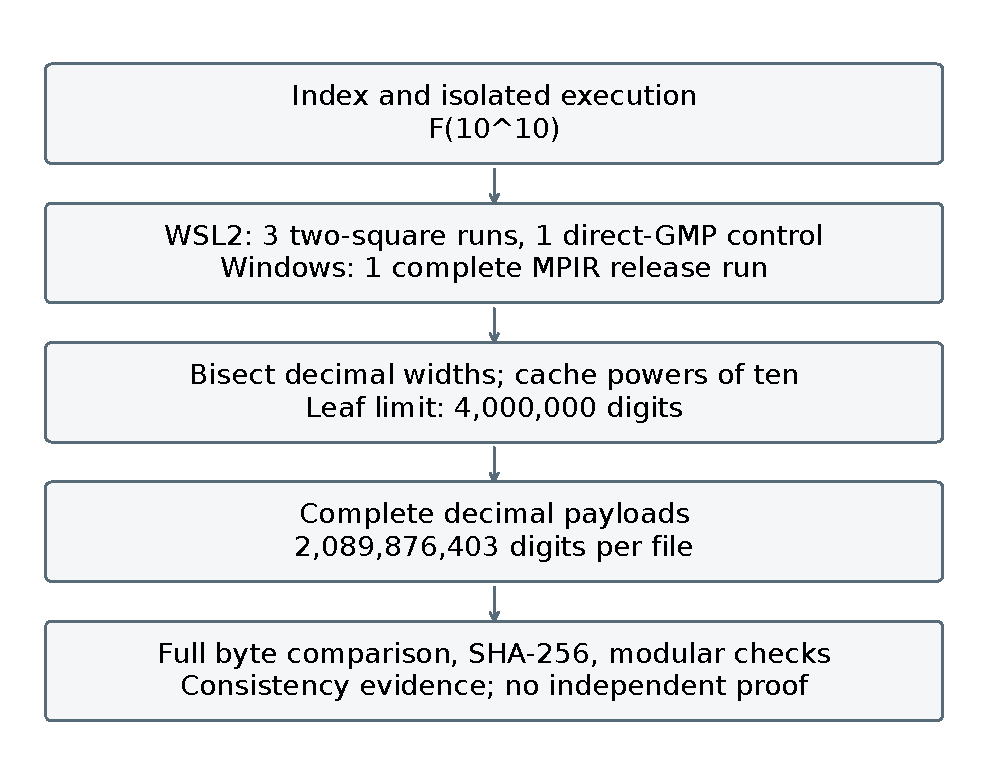
\includegraphics[width=0.64\linewidth]{figures/architecture_en.pdf}
\caption{Measured execution and verification workflow. Trial counts distinguish two-square runs from the direct-library control; agreement checks are not an independent correctness proof.}
\end{figure}

\section{Evidence and experimental setting}

Experiments were run on 15 October 2026 on an Intel Core i5-14400F host with 10 physical cores, 16 logical processors and 34,072,674,304 bytes of visible physical memory. Windows reported build 27766. The failing native path used Python 3.13.7 and gmpy2 2.3.1 with GMP 6.3.0; a downloaded PyPI wheel (SHA-256 \texttt{74235fcce8a1bee2\allowbreak{}07bf8d43955cb045\allowbreak{}63f71ba8231a3bba\allowbreak{}fc6dd7869503d05c}) supplied gmpy2 2.2.1 for two further failure trials. Its bundled `libgmp-10.dll` has SHA-256 `\texttt{fb2d312ca861c18e\allowbreak{}8b23648ac8440b0b\allowbreak{}613b1930ceff58f4\allowbreak{}8b48ba2d3bd6b186}`, distinct from the 2.3.1 DLL. Both report GMP 6.3.0; compiler and build flags are not established by wheel metadata. WSL2 Ubuntu used Python 3.12.3, gmpy2 2.1.5 and GMP 6.3.0, with a 5.15.167.4 WSL2 kernel. Its visible memory was 16,240,976 KiB and swap 4 GiB. These are distinct runtime builds, not an operating-system-only controlled comparison. Raw environment records accompany every Linux trial.

The archived Python v4.3 source has SHA-256 \texttt{f40028d222e33178\allowbreak{}aff8fd27714c4642\allowbreak{}bb2510d8cd23e191\allowbreak{}6587f948b7ee108b}. It matches the pinned Git source after LF/CRLF normalization. The arithmetic and decimal-writer functions were imported without changing their formulas. A separate driver supplied native GMP, conventional fast doubling, Lucas and two-square runs. Each algorithm was measured five times at $n=10^{7}$, $10^{8}$, $5\times 10^{8}$ and $10^{9}$, in fresh processes with a cyclically rotated order. All benchmark processes ran sequentially; normal host background activity was not eliminated. Arithmetic timing disables the application diagnostics callback (diag=None); it excludes module import and process startup. Timed results therefore do not include the original worker's per-layer diagnostic logging. Main tables report medians; supplementary arithmetic\_summary.csv supplies inclusive linearly interpolated quartiles and ranges; no significance test is inferred from five observations.

Three WSL2 two-square trials at $n=8\times 10^{9}$ tested the former failure scale without decimal output. Three complete $n=10^{10}$ WSL2 two-square runs were recorded, with one complete native Windows MPIR v1.1.0 release run following the first Linux trial. A final Linux native gmpy2.fib call generated a new reference at $n=10^{10}$, bypassing the application's Windows-derived dispatch cutoff. The MPIR executable is identified by SHA-256 \texttt{bda33f884b986765\allowbreak{}48124096be8e747a\allowbreak{}336330355e6c8a34\allowbreak{}acaf882cd9f50921}; its bytes were tested directly. Current C source, an older C snapshot and the release executable are distinguished rather than assumed to be one rebuilt object.

Linux perf\_counter intervals separate arithmetic from decimal conversion and file close. The instrumented driver writes an ASCII digit-only payload using the original writer. An explicit fsync interval is recorded afterwards and excluded from conversion time; verification is timed separately. Linux resource.getrusage and /usr/bin/time -v record kernel cumulative process peak RSS. The arithmetic checkpoint and full-run peak are cumulative high-water values, not disjoint per-stage peaks. Native MPIR is timed externally from process creation to termination; its stdout stage timings have one-second granularity and are not substituted for the precise Linux intervals. Windows memory is sampled every 50 ms and includes the operating system's peak-working-set and peak-pagefile counters up to the last successful query. A final short-lived peak after that query cannot be excluded. Working set, RSS and private commitment are reported under their own names.

Each Linux result is checked modulo 1,000,000,007, 1,000,000,009, 2,147,483,647 and $10^{100}$ by a bounded-integer fast-doubling implementation. These checks test arithmetic consistency but do not prove every digit correct. The new native reference was streamed once more: decimal digit sums gave mod 9 = 6 and mod 11 = 0, matching bounded Fibonacci residues. Cassini's identity held modulo 1,000,000,007, 1,000,000,009 and 2,147,483,647; a period-based check gave last five digits 46875 and a separate 90-digit logarithm gave first five digits 14135. The other four new payloads share the reference's SHA-256. Each complete output is counted, checked for non-digits and hashed in bounded chunks. Primary byte comparisons use the new native GMP file and the four new repair-path outputs, removing documented headers and ASCII whitespace. Retained 2024 artifacts are compared separately for the historical audit. Full agreement is a stronger artifact check than endpoints alone; shared algorithms and libraries still limit implementation independence.

\section{Results}

\subsection{Repeated arithmetic comparisons}

At $n=10^{9}$ the five-trial arithmetic medians were native GMP 3.844 s, two-square 4.610 s, Lucas 5.622 s and conventional doubling 7.844 s.

\begin{table}[htbp]
\centering\small
\caption{Five-trial arithmetic medians}
\begin{tabularx}{\linewidth}{lXXXX}
\toprule
Index n & Native / s & Doubling / s & Lucas / s & Two-square / s \\
\midrule
$10^{7}$ & 0.022 & 0.044 & 0.033 & 0.026 \\
$10^{8}$ & 0.334 & 0.659 & 0.483 & 0.400 \\
$5\times 10^{8}$ & 2.015 & 4.013 & 2.927 & 2.359 \\
$10^{9}$ & 3.844 & 7.844 & 5.622 & 4.610 \\
\bottomrule
\end{tabularx}
\end{table}

Note: Five fresh-process trials per algorithm and scale; only medians appear here. Linearly interpolated Q1, Q3, IQR and ranges are supplied in arithmetic\_summary.csv.

\begin{figure}[htbp]
\centering
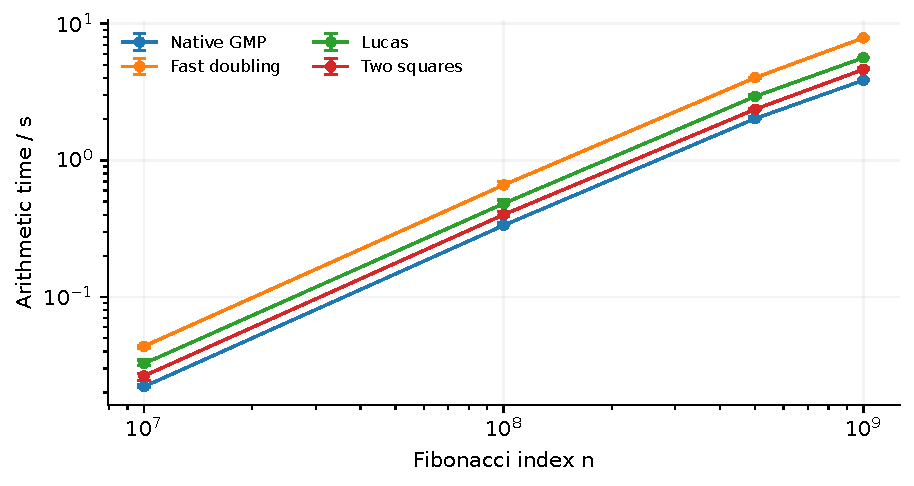
\includegraphics[width=0.92\linewidth]{figures/benchmark_en.pdf}
\caption{Arithmetic medians with interquartile ranges, five fresh-process trials per algorithm and scale.}
\end{figure}

\subsection{Failure and repair paths}

\subsubsection{Failure observations}

The two native gmpy2 2.3.1 trials and two isolated gmpy2 2.2.1 trials failed at layer 32/32, the first square of a 2,776,967,654-bit operand, before decimal conversion. The preserved stderr contains GNU MP: Cannot allocate memory (size=4294597664). The current 2.3.1 trials exited with code 3 rather than the historical report's 0xC0000409. No watchdog termination was involved. Median peak working set and private commitment were 1.82 and 2.46 GiB for gmpy2 2.3.1, and 1.81 and 2.46 GiB for 2.2.1, respectively; these are distinct Windows counters. In the two gmpy2 2.3.1 runs, more than 10 GiB of physical memory remained available at the last pre-failure diagnostic. Available physical memory alone does not identify the failure; the full-width allocation trace and isolated tests below resolve the nature of the requested size.

\subsubsection{Full width allocation trace}

A separate allocator trace delegated to the original GMP allocation functions and recorded full-width size\_t arguments before gmpy2 initialization. Its allocation values and log are supplied separately; traced timings are excluded from performance summaries. The largest recorded request was 18,446,744,073,709,181,984 bytes. This near-limit 64-bit size\_t value has low 32 bits equal to 4,294,597,664, matching the displayed stderr size. The request equals $2^{64}$ minus 369,632 bytes; interpreted as a signed 64-bit integer, the same bit pattern is -369,632.

\subsubsection{Minimal reproduction and build comparison}

In protected processes on 16 October 2026, sparse operands with only the highest bit set showed adjacent square outcomes at b=2,147,352,576 and b=2,147,352,577. Define T=$2^{32}$\ensuremath{-}$2^{18}$=4,294,705,152 bits and L=T/64=$2^{26}$\ensuremath{-}$2^{12}$=67,104,768 limbs. The successful mathematical square has T\ensuremath{-}1 bits and the failed one T+1 bits. This is an observed sparse-square transition, not a universal minimum for other operand shapes. The direct DLL test and separately compiled C reproducer use the following core operations; each case runs in its own guarded process.

\begin{quote}\footnotesize
\begin{verbatim}
mpz_t x, y;
mpz_init_set_ui(x, 1);
mpz_init(y);
mpz_mul_2exp(x, x, b - 1);
mpz_mul(y, x, x);
mpz_clear(y);
mpz_clear(x);
\end{verbatim}
\end{quote}

The two wheel binaries are identified as `\path{site-packages/gmpy2.libs/libgmp-10.dll}`: gmpy2 2.3.1 SHA-256 `\texttt{829adcf025d22e64\allowbreak{}1c6816b431fbe5b2\allowbreak{}26a39b390c720519\allowbreak{}2d480151646fe9c9}` and gmpy2 2.2.1 SHA-256 `\texttt{fb2d312ca861c18e\allowbreak{}8b23648ac8440b0b\allowbreak{}613b1930ceff58f4\allowbreak{}8b48ba2d3bd6b186}`. An independent MSYS2 mingw-w64-x86\_64-gmp 6.3.0-2 package \cite{msys2_gmp} supplies a third DLL, `\path{mingw64/bin/libgmp-10.dll}`, SHA-256 `\texttt{37248cda33845e7c\allowbreak{}5c35a574e57da762\allowbreak{}dd0a8268f0270d17\allowbreak{}9f30a33746809681}`. Its verified package SHA-256, CI packager, build date and GCC 13.2.0-2 build-environment record are supplied. All three reproduced the adjacent pair. At b=2,147,352,577, the 2.3.1 DLL requested $2^{64}$\ensuremath{-}523,232 bytes; the 2.2.1 DLL requested $2^{64}$\ensuremath{-}523,232 bytes; the MSYS2 DLL requested $2^{64}$\ensuremath{-}523,232 bytes. These requests were captured by native C allocation callbacks forwarding to each DLL's original allocator.

\begin{table}[htbp]
\centering\small
\caption{Adjacent sparse-square outcomes in all three tested DLLs}
\begin{tabularx}{\linewidth}{lXXXX}
\toprule
Operand bits b & Result bits & Delta from T & 64-bit limbs & Observed result \\
\midrule
2,147,352,576 & 4,294,705,151 & \ensuremath{-}1 & 67,104,768 & Succeeded \\
2,147,352,577 & 4,294,705,153 & +1 & 67,104,769 & Wrapped request \\
\bottomrule
\end{tabularx}
\end{table}

The delta column is mathematical result bits minus T. Result widths in failed cases follow from the sparse inputs; no failed result object was recovered. Limbs in this table describe the normalized mathematical result, not an observed FFT workspace length.

\subsubsection{Scope and mechanism tests}

A separate C probe compiled against the matching MSYS2 package header measured sizeof(mp\_limb\_t)=8, sizeof(mp\_size\_t)=4, sizeof(mp\_bitcnt\_t)=4 and sizeof(unsigned long)=4 bytes. The two wheel headers were not recovered, so their typedef widths are not established by this header probe. The inspected MPIR Win64 header instead defines 64-bit mp\_size\_t and mp\_bitcnt\_t \cite{mpir}. Thus type widths differ across these builds. This makes 32-bit length or workspace arithmetic a testable hypothesis; a header width alone does not identify which internal operation produced the request. GMP's mpz\_t capacity fields count limbs \cite{gmp_internals}, and approximately 67 million limbs remain far below INT\_MAX.

Sofroniou of Wolfram Research reported a GMP 5.1.2 failure on 64-bit Linux: an int multiplication of K and l overflowed before assignment to mp\_size\_t, then reached allocation as a huge size\_t \cite{gmp_size_overflow}. That historical mechanism motivates checking intermediate arithmetic, rather than assigning its source expression to the present DLLs.

At six sampled square widths from 2,147,352,577 through 2,147,483,648 bits, the signed interpretation of the abnormal request stayed at \ensuremath{-}523,232 bytes. At 2,776,967,654 bits it was \ensuremath{-}369,632 bytes. Both are multiples of the 8-byte limb size, corresponding arithmetically to \ensuremath{-}65,404 and \ensuremath{-}46,204 limb-sized units; this does not prove an internal variable held either negative limb count. The plateau does not support a single nonconstant affine request-versus-raw-bit formula over those samples.

Distinct-address multiplication with unequal operand lengths also failed when the mathematical result had exactly T bits. A stronger matched-result test used bit-length pairs (2,147,352,513, 2,147,352,577) and (2,147,352,512, 2,147,352,578). Both mathematical products have 4,294,705,089 bits and 67,104,768 normalized limbs; their input limb sums are respectively 67,104,769 and 67,104,768. The former failed with the wrapped request and the latter succeeded in all three DLLs. These tests rule out mathematical result width or normalized result limb count as the sole trigger in these cases, and show that a square-specific path is not required. Input limb lengths and internal padding/workspace handling are therefore the next quantities to trace. Internal FFT lengths and the first overflowing expression remain unmeasured. All Windows tests used build 27766; no stable-Windows replication has been obtained.

At the same Fibonacci index, WSL2 two-square completed all three trials, with median arithmetic time 48.18 s and median peak RSS 2.81 GiB. The native Windows MPIR release also completed the larger $n=10^{10}$ full-output task once; the instrumented MPIR build completed three arithmetic trials at each of $n=8\times 10^{9}$ and $n=10^{10}$. These observations demonstrate two usable execution paths around the observed failure. They do not constitute a patch to the original GMP binary, nor establish that all Windows GMP builds fail or that all Linux builds succeed.

\subsection{Complete decimal output}

For $n=10^{10}$, WSL2 two-square arithmetic had median 56.95 s and conversion with file close median 551.98 s; the median sum of those measured stages was 608.93 s. The median output-stage share was 90.65\%. Individual trials, explicit fsync intervals and full ranges are retained in the supplementary CSV. The median cumulative full-run peak RSS was 5.10 GiB. The historical 53.6 s, 527.8 s and approximately 5 GiB estimate remain archival observations and are superseded by the new protocol for current performance claims.

One native Windows MPIR v1.1.0 full-output run completed with external process wall time 2592.93 s and observed peak working set 8.05 GiB. Its total includes the program's width correction, initialization, progress thread and file close; no durable-file-sync measurement was added to the release executable. Because this endpoint differs from the Linux stage sum, these endpoints are not presented as a controlled implementation speedup. In particular, Python/WSL2 timings are not attributed to MPIR.

\begin{table}[htbp]
\centering\small
\caption{New complete Linux output trials}
\begin{tabularx}{\linewidth}{lXXXX}
\toprule
Run & Arithmetic / s & Output / s & Stage sum / s & Peak RSS / MiB \\
\midrule
Native & 48.12 & 542.81 & 590.94 & 5219.6 \\
2S-1 & 58.60 & 557.22 & 615.81 & 5219.7 \\
2S-2 & 53.88 & 548.49 & 602.37 & 5219.4 \\
2S-3 & 56.95 & 551.98 & 608.93 & 5221.6 \\
\bottomrule
\end{tabularx}

\end{table}

Note: Native is one direct gmpy2.fib control in the same WSL2/Linux environment. It is excluded from the 2S-1/2/3 medians, quartiles and figure error bars. Columns are rounded independently to two decimal places; stage sums use unrounded intervals, so adding displayed components can differ by 0.01 s. Peak is cumulative RSS; fsync and verification are separate.

\begin{figure}[htbp]
\centering
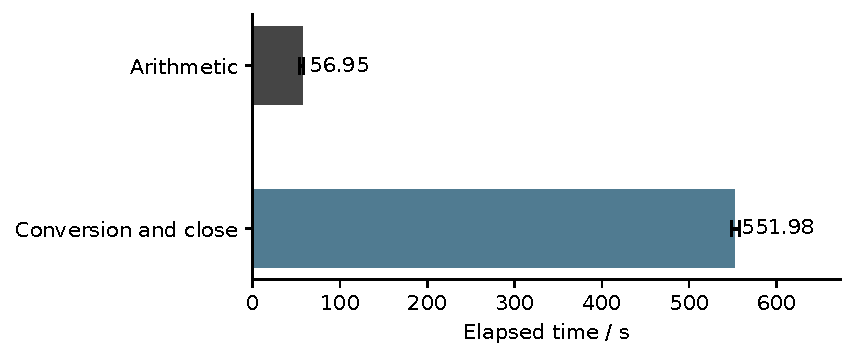
\includegraphics[width=0.92\linewidth]{figures/stages_en.pdf}
\caption{Three WSL2 two-square full-output trials at $n=10^{10}$; bars are medians and error bars the observed range. The Native control is excluded. Conversion includes close; fsync is separate.}
\end{figure}

\subsection{Verification and reference provenance}

All five newly generated files contain 2,089,876,403 decimal digits. The digit-only payloads agree in SHA-256 and full byte comparison after the MPIR prefix is removed. Their common digest is shown below.

\begin{center}\ttfamily\small
6fa62cdd9d65374354899719d9a58122\\
2c1d497492b9bcddcb859c32bc469662
\end{center}

The first five digits are 14135 and the last five 46875. The new reference is an author-generated result of the direct Linux GMP API, with its source, command, runtime versions, environment, original stdout and resource record supplied. It provides a reproducible generation chain without relying exclusively on the old external attribution. It is not a third-party certified standard or an independent-library result. Historical files are audited only for continuity with retained material and are not primary validation evidence. Their original machine, generation command and third-party provenance remain unauthenticated; details are supplied in historical\_provenance.md.

\begin{table}[htbp]
\centering\small
\caption{New output and reference verification}
\begin{tabularx}{\linewidth}{lX}
\toprule
Check & Result \\
\midrule
New complete payloads & 3 WSL2 + 1 MPIR + 1 native reference \\
Digits per payload & 2,089,876,403 \\
New native reference & Linux gmpy2.fib \\
Full comparison & MATCH \\
SHA-256 & Identical; see text \\
First / last 5 digits & 14135 / 46875 \\
Date & 2026-10-15 \\
\bottomrule
\end{tabularx}
\end{table}

\subsection{Native Windows MPIR repeated measurements}

The retained C and Python writers both use 4,000,000-digit leaves, but C calls MPIR mpz\_tdiv\_qr/mpz\_get\_str and fwrite whereas Python calls GMP f\_divmod/digits and writes through a Python file object. The MPIR release also performs width correction and status reporting. Linux output was written under WSL2 /tmp and Windows output to C:. Conversion, padding, runtime I/O and storage waits were not measured separately, so the timing gap cannot be attributed to any one of them. Retained C source is not a binary-matched rebuild of the release.

The sampling protocol was amended after the first MPIR full-output run revealed a much longer conversion stage. The target release run was preserved, while repetition was concentrated on five complete $n=10^{9}$ MPIR runs and three arithmetic-only trials at each of $n=8\times 10^{9}$ and $n=10^{10}$. The compute-only executable was rebuilt from the retained C snapshot with QueryPerformanceCounter around the unchanged Fibonacci function and an exit branch before decimal conversion. Its source, build command, library hash and executable hash are supplied separately from the release. Arithmetic medians were 107.97 s and 122.22 s at the two large indices. At $n=10^{10}$, 122.22 s is about 2.15 times the WSL2 two-square median of 56.95 s; this descriptive build comparison does not isolate an operating-system effect. The single complete MPIR target run is not presented as a repeated full-output statistic. The first release run's sampler was replaced while preserving its numeric process; the protocol amendment and both memory traces are retained, and that run's wall clock uses the operating-system process creation timestamp to observed exit.

Follow-up sink controls used $n=10^{9}$ and three fresh-process trials per condition, with the second round reversing condition order. The unchanged MPIR release had median process wall times 197.00 s to a C: file and 199.37 s to NUL (NUL/file=1.012). The unchanged Linux writer had median conversion-and-close times 37.90 s under WSL2 /tmp and 40.30 s under /mnt/c (/mnt/c-to-/tmp=1.063); fsync remained separate. MPIR includes arithmetic, width correction and status output, so cross-backend endpoints still differ. The stored control files matched by SHA-256; NUL produced no numeric artifact. These are within-backend sink comparisons at one billion, without a target-scale decomposition of the ten-billion timing gap.

\begin{table}[htbp]
\centering\small
\caption{MPIR measurements by endpoint and sample size}
\begin{tabularx}{\linewidth}{lXXXX}
\toprule
Index & Mode & Trials & Time / s & Peak WS / GiB \\
\midrule
$10^{9}$ & Full & 5 & 185.50 & 0.78 \\
$8\times 10^{9}$ & Compute & 3 & 107.97 & 5.18 \\
$10^{10}$ & Compute & 3 & 122.22 & 6.47 \\
$10^{10}$ & Full & 1 & 2592.93 & 8.05 \\
\bottomrule
\end{tabularx}
\end{table}

\section{Reproduction procedure}

Run the supplementary driver with its pinned source snapshot, recording the installed library builds before any target-scale run. Small inputs should first agree with known values, including $F(100)$=354224848179261915075. The supplementary Linux worker accepts an explicit algorithm, mode, index and output directory; the experiment controller records the exact invocation for each trial.

The public application can also be executed directly in worker mode. Its default Linux dispatch retains the conservative Windows threshold; direct native-GMP comparison is selected by the supplementary driver rather than by silently changing the application.

\begin{quote}\footnotesize
\begin{verbatim}
python3 fibonacci_calculator_v4_3.py \
  --worker 100 full auto \
  F_100.txt diagnostic_100.log v1
\end{verbatim}
\end{quote}

\begin{quote}\footnotesize
\begin{verbatim}
python3 fibonacci_calculator_v4_3.py \
  --worker 10000000000 full auto \
  F_10000000000_linux.txt diagnostic.log v1
\end{verbatim}
\end{quote}

Keep the result header policy explicit when verifying an application-produced file. The new benchmark driver writes only ASCII digits; the original worker writes two metadata lines, while the MPIR release writes a fixed $F(n)$ prefix. The verification manifest records the exact offsets and comparisons. Raw outputs are kept in distinct directories and do not overwrite historical artifacts.

\section{Limitations and discussion}

The study uses one host and recorded builds. Five small-scale repeats and three Linux full-scale repeats describe local variability, without establishing population-level performance or asymptotic superiority. Host background activity and file caches were not controlled through dedicated-machine isolation; the fixed rotated algorithm order was not randomized. Linux and Windows resource endpoints differ, and cumulative kernel peaks cannot locate every allocation's contribution. The separate allocator trace changes instrumentation and is excluded from untraced timing summaries.

The wrapped allocation size is established by the full-width callback and direct DLL probe; the responsible source expression has not been established by a binary-matched source build or native stack analysis. A successful replacement backend demonstrates an operational remedy, not correction of that expression. The new reference has a documented generation chain but shares GMP and established identities with one test path. Modular checks and cross-backend agreement reduce several error risks without providing formal verification. The 2024 file's original supercomputer execution and redistribution rights remain unverified, and a public archival DOI for the new data has not been assigned.

\section{Conclusion}

New experiments demonstrate a reproducible native Windows GMP failure and two completed large-integer output paths on the recorded home computer. Three WSL2 runs and one native MPIR release run each produced the complete ten-billionth Fibonacci number, with recorded runtime and memory evidence and full agreement with a newly generated native GMP reference. Decimal conversion accounts for a median 90.65\% of the WSL2 stage total. In this experiment, backend selection, temporary-memory handling and output engineering determine whether an established arithmetic algorithm can deliver a complete artifact. Broader platform claims and the specific overflowing source expression require additional controlled evidence.

Full output agrees with direct library evaluation, and modular checks satisfy the tested arithmetic relations. This is consistency evidence: the Linux paths share GMP and established identities, and matching SHA-256 digests do not independently prove numerical correctness. No independent implementation or formal correctness proof is provided.

\section{Availability and author declarations}

The software remains MIT-licensed at the pinned public Git revision \cite{software}. Supplementary experiment drivers, raw measurements, environment files, source and binary hashes, failure diagnostics, the isolated square/direct-DLL probes of 16 October 2026, numeric verification manifests and the reference-generation command are supplied with this revision. The new full numeric outputs are retained locally and identified by file hashes; the package does not claim that a public archive or DOI already exists. Historical files retain their original provenance qualifications. Software citation follows version-specific identification \cite{citation}.

Xudong Lu is the author and corresponding author, affiliated with Fengjing High School Affiliated to East China Normal University, Shanghai, China; correspondence: lusunrise@126.com. AI tools assisted code development, experimental orchestration and evidence processing, and manuscript preparation and translation. The author is responsible for scientific judgment, evidence verification, and the final submission text, and takes responsibility for all content in the manuscript. AI systems are not listed as authors.

\begin{thebibliography}{99}
\raggedright
\bibitem{brent} Brent RP, Zimmermann P. 2010. Modern Computer Arithmetic. Cambridge University Press. \url{https://doi.org/10.1017/CBO9780511921698}

\bibitem{gmp_fib} The GNU MP developers. 2023a. Fibonacci Numbers Algorithm. GNU MP 6.3.0 manual. \url{https://gmplib.org/manual/Fibonacci-Numbers-Algorithm}

\bibitem{gmp_fft} The GNU MP developers. 2023b. FFT Multiplication. GNU MP 6.3.0 manual. \url{https://gmplib.org/manual/FFT-Multiplication}

\bibitem{software} Lu X. 2026. Fibonacci 10 Billion Calculator. Python v4.3, Git revision f0c5f2488432524d6edb781cbabe1bbca2a79b6d. MIT license. \url{https://github.com/sr-lxd/fibonacci-10-billion-calculator/tree/f0c5f2488432524d6edb781cbabe1bbca2a79b6d}

\bibitem{gmp_size_overflow} Sofroniou M. 2013. mpn\_mul\_fft type overflow issue. GMP developers mailing list, 18 September 2013. \url{https://gmplib.org/list-archives/gmp-devel/2013-September/003365.html}

\bibitem{gmp_mpz} The GNU MP developers. 2023d. Number Theoretic Functions. GNU MP 6.3.0 manual. \url{https://gmplib.org/manual/Number-Theoretic-Functions}

\bibitem{mpfr_paper} Fousse L, Hanrot G, Lefèvre V, Pélissier P, Zimmermann P. 2007. MPFR: A multiple-precision binary floating-point library with correct rounding. ACM Transactions on Mathematical Software 33(2):13. \url{https://doi.org/10.1145/1236463.1236468}

\bibitem{mpfr_manual} The MPFR developers. 2025. GNU MPFR 4.2.2 manual. \url{https://www.mpfr.org/mpfr-current/mpfr.html}

\bibitem{gmpy2_mpz} The gmpy2 contributors. n.d. Multiple-precision integers. gmpy2 documentation. Accessed 14 October 2026. \url{https://gmpy2.readthedocs.io/en/latest/mpz.html}

\bibitem{gmp_radix} The GNU MP developers. 2023e. Binary to Radix. GNU MP 6.3.0 manual. \url{https://gmplib.org/manual/Binary-to-Radix}

\bibitem{gmp_memory} The GNU MP developers. 2023c. Memory Management. GNU MP 6.3.0 manual. \url{https://gmplib.org/manual/Memory-Management}

\bibitem{python_subprocess} Python Software Foundation. n.d.-a. subprocess: Subprocess management. Python 3.13 documentation. Accessed 14 October 2026. \url{https://docs.python.org/3.13/library/subprocess.html}

\bibitem{msys2_gmp} MSYS2. n.d. mingw-w64-x86\_64-gmp 6.3.0-2 package and build metadata. Accessed 16 October 2026. \url{https://packages.msys2.org/packages/mingw-w64-x86_64-gmp}

\bibitem{mpir} The MPIR contributors. n.d. MPIR Windows source and Win64 definitions. Inspected revision 5e0c2061af105c151970d41c8394ce956f77e455. \url{https://github.com/BrianGladman/mpir/blob/5e0c2061af105c151970d41c8394ce956f77e455/gmp-h.in}

\bibitem{gmp_internals} The GNU MP developers. 2023f. Integer Internals. GNU MP 6.3.0 manual. \url{https://gmplib.org/manual/Integer-Internals}

\bibitem{citation} Smith AM, Katz DS, Niemeyer KE, FORCE11 Software Citation Working Group. 2016. Software citation principles. PeerJ Computer Science 2:e86. \url{https://doi.org/10.7717/peerj-cs.86}

\end{thebibliography}
\end{document}
